\section{Introduction}\label{sec:introduction}

\subsection{Contexte : le projet Sailowtech}

\begin{figure}[H]
  \centering
  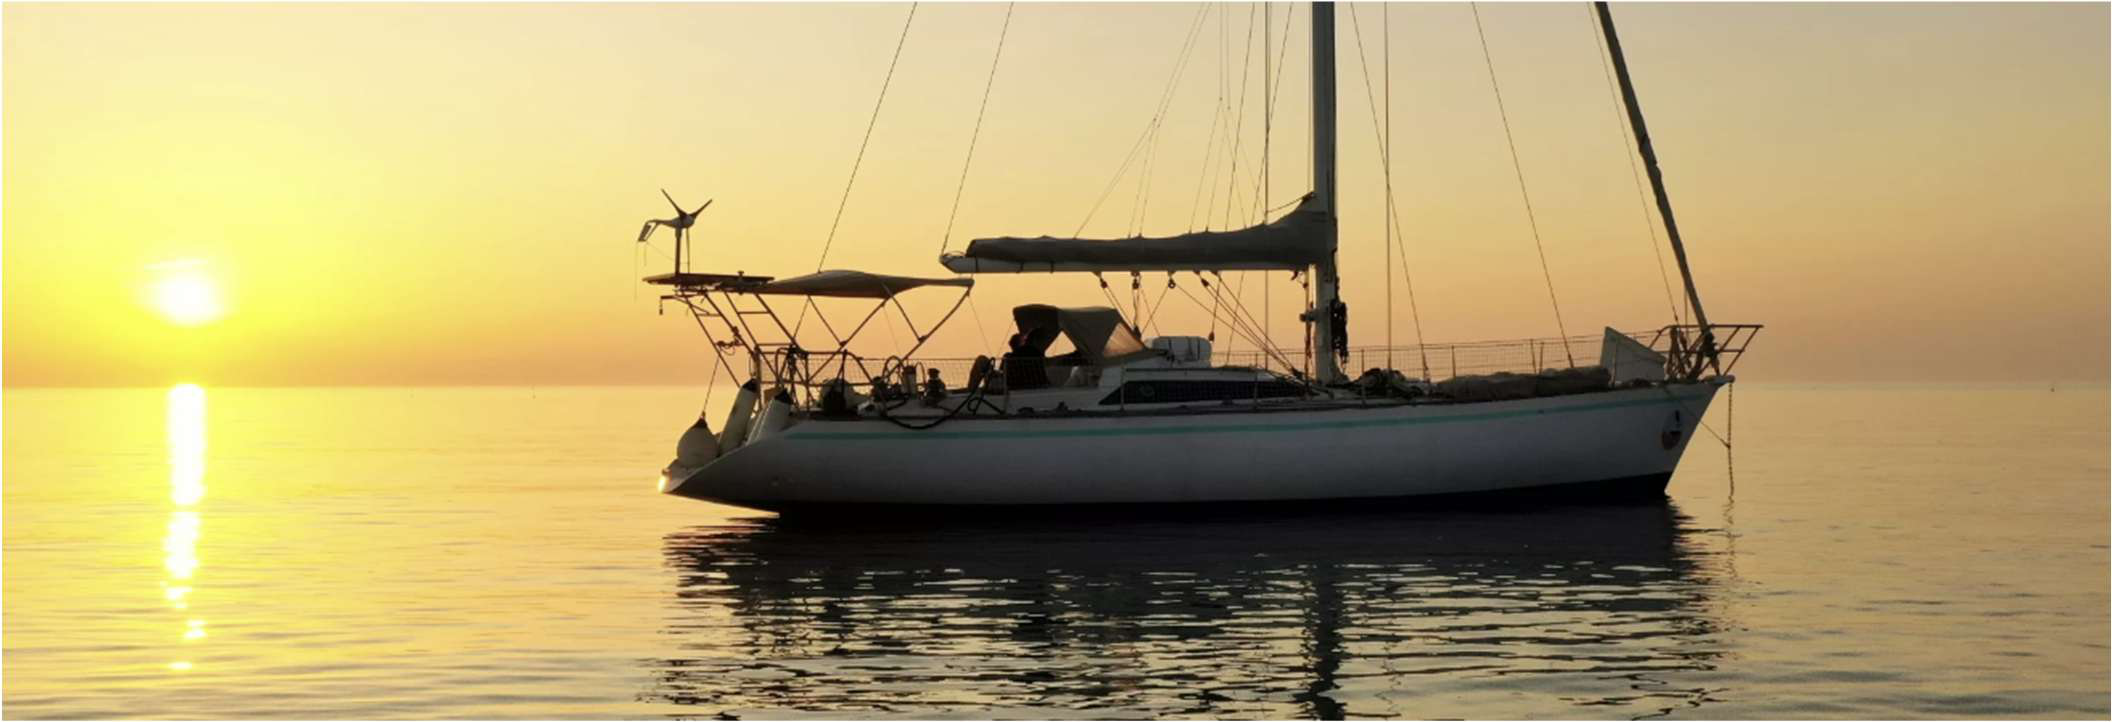
\includegraphics[width=0.7\textwidth]{images/voilier_sunset.png}
  \caption{Un voilier équipé de la station Sailowtech en expédition.}
  \label{fig:voilier}
\end{figure}

\textit{Sailowtech} est une initiative dont l'objectif est de rendre l'océanographie
plus accessible et durable en équipant les expéditions à la voile d'innovations à
bas coût. L'idée centrale est de transformer des voiliers ordinaires en plateformes
de collecte de données scientifiques, sans alourdir les équipages de technologies
complexes ou coûteuses. Les données ainsi récoltées --- qualité de l'air, paramètres
de la colonne d'eau, couverture nuageuse --- alimentent des bases de données
scientifiques ouvertes sur les océans.

\subsection{Objectifs du projet}

Notre projet de semestre ME-401, supervisé par Eric Boillat du Laboratoire de
Métallurgie Thermomécanique (LMTM) de l'EPFL, consiste à concevoir et réaliser
une station météo embarquée adaptée aux contraintes d'une expédition maritime.
La station doit remplir plusieurs fonctions :

\begin{itemize}
  \item \textbf{Acquisition de données atmosphériques} : mesure des particules
    fines (PM$_{1.0}$, PM$_{2.5}$, PM$_{10}$), de l'irradiance solaire,
    de la température, de la pression et de l'humidité.
  \item \textbf{Intégration au réseau du bateau} : réception et coordination
    des données provenant d'une sonde CTD (Conductivité, Température, Profondeur)
    sous-marine et, potentiellement, du logiciel de navigation Garmin.
  \item \textbf{Résistance aux conditions marines} : protection contre les
    projections d'eau, la corrosion saline et les vibrations.
  \item \textbf{Autonomie énergétique} : alimentation par batterie avec
    régulation DC-DC embarquée.
  \item \textbf{Vision par ordinateur (bonus)} : détection automatique de la
    couverture nuageuse par analyse d'images.
\end{itemize}

\subsection{Répartition du travail}

La réalisation du projet a été partagée entre les deux membres de l'équipe :

\begin{itemize}
  \item \textbf{Design électronique} : Guilhem Destriau (responsable principal)
    et Romain Corbel.
  \item \textbf{Design mécanique} : Romain Corbel (responsable principal)
    et Guilhem Destriau.
\end{itemize}
